\section{问题二：第二检测点的主动选择}
\label{sec:q2}

\subsection{首次观测区域与保证接收的候选区域}
问题二要求根据全向源的一次示向读数选择第二检测点，使交会定位获得较好的效果，并给出候选区域。题面并未强制要求第二点对所有允许目标位置均能接收信号；本文将这一条件作为保守的选点约束。记首个检测点为 $s_0$、示向度为 $\theta_0$，显式利用目标圆域及有效接收半径上界，可得连续位置集合
\begin{equation}
 \Omega_1=B(0,1800)\cap W(s_0,\theta_0,\delta)\cap B(s_0,1500).
 \label{eq:q2-prior}
\end{equation}
程序按照问题一的外包方式构造多边形 $P_1\supseteq\Omega_1$，本节数值算例使用几何函数默认误差 $\delta_{\rm impl}=1.00500001^\circ$。已获得有效示向读数还意味着距离大于 $5\,\mathrm m$，但当前多边形实现没有减去近距离圆盘；保留这部分位置使集合更保守，并保持凸性。

有效接收半径未知但至少为 $1000\,\mathrm m$，因而对全向源，可以采用
\begin{equation}
 \mathcal C_{\rm safe}(P_1)
 =\bigcap_{p\in P_1}B(p,1000)
 =\bigcap_{v\in V(P_1)}B(v,1000)
 =\left\{s:\max_{v\in V(P_1)}\|s-v\|\leq1000\right\}.
 \label{eq:q2-safe}
\end{equation}
等式由凸集顶点的距离充分性得到：若 $p=\sum_i\alpha_i v_i$，则 $\|s-p\|\leq\sum_i\alpha_i\|s-v_i\|\leq1000$。所以该区域为凸圆盘交集，对其中任意检测点和 $P_1$ 中任意目标位置，均满足最小有效接收半径约束。由于使用的是外包多边形，这只是保证接收的充分候选区域；区域外也可能接收到实际目标信号。

保证接收不等于保证返回示向度。附件规定，当距离不超过 $5\,\mathrm m$ 时返回近距离信息，可直接进入光学精确定位和清除；此时不返回方位角。本节的几何评分预测的是有示向度时的交会结果，未显式评价该近距离分支。因此，接收可行性与后验评分精度是两项不同的性质。程序按全部顶点距离不超过 $1000$ 进行浮点筛选，没有额外缩小阈值，也不将其声称为任意边界输入下的精确算术证明。

\subsection{交会几何与有限候选点}
只沿第一次示向线移动，通常不能显著增加两次观测的交会角；移向示向线侧方则可能使交会区域在两个方向同时收缩。局部线性化时，角误差对应的横向偏差随距离增大，而交会角过小会放大位置不确定性。较接近直角的交会可改善局部条件，但目标位置本身未知，长距离横移还增加耗时，故不能把 $90^\circ$ 当作独立于距离、误差与动作时间的全局最优条件。主动选择测点与权衡移动、测量成本可参考文献\cite{tokekar2011,vanderhook2014}；这些文献的观测假设及性能保证并不自动适用于本题。

以首测示向为横轴生成网格，记二维旋转矩阵为 $R(\theta_0)$，候选集合写为
\begin{equation}
 \begin{split}
 \mathcal S_{\rm grid}=
 \{s_0+R(\theta_0)(a,b)^{\mathsf T}:\ &a=0,50,\ldots,1500,\\[-2pt]
                                      &b=-600,-560,\ldots,600\},\\
 \mathcal S=\mathcal S_{\rm grid}\cap\mathcal C_{\rm safe}(P_1).
 \end{split}
 \label{eq:q2-grid}
\end{equation}
该式是现有 $s_0=(0,0)$ 算例的坐标表达，原入口固定首测点为原点、首测示向度为 $30^\circ$，不应据此声称已实现任意首测输入的通用命令接口。原始网格共有 $31\times31=961$ 个点，已有结果保留 $213$ 个安全候选点。有限网格仅用于数值搜索，不等同于连续候选区域本身。通用选点辅助函数还提供围绕几何中心与长轴生成候选点的方式，但本例显式传入上述网格，没有使用该默认候选生成器。

\subsection{采样后验直径与动作时间评分}
对于候选点 $s$，理想的稳健评价需考虑 $P_1$ 内所有目标位置及全部允许测向误差，计算第二次观测后定位直径的最大值。当前实现用有限情景近似该问题。先取多边形顶点及顶点坐标的算术均值作为位置代表；若代表数超过 $9$，按数组索引等距抽取 $9$ 个。这里的算术均值不是多边形面积质心，也不是目标位置的概率期望。将代表集合记为 $\mathcal G$，误差代表为
\begin{equation}
 \mathcal E=\{-\delta_{\rm impl},0,\delta_{\rm impl}\}.
\end{equation}
令 $\operatorname{atan2}_{\deg}=(180/\pi)\operatorname{atan2}$ 表示以度为单位的方位角。对每个 $(g,e)\in\mathcal G\times\mathcal E$，构造预测示向度
$\widehat\theta(s;g,e)=\operatorname{atan2}_{\deg}(g_y-s_y,g_x-s_x)+e$，并定义
\begin{equation}
 \begin{split}
 P_2(s;g,e)&=P_1\cap W(s,\widehat\theta(s;g,e),\delta_{\rm impl}),\\
 \widehat D_{\rm worst}(s)&=
 \max_{\substack{g\in\mathcal G,\ e\in\mathcal E\\P_2(s;g,e)\ne\varnothing}}
 D\bigl(P_2(s;g,e)\bigr).
 \end{split}
 \label{eq:q2-sampled}
\end{equation}
这里的“最坏”仅指已采样情景中的最大值。取多边形顶点足以计算固定圆心的最远距离，但不意味着顶点及三种误差足以实现非线性的连续最坏后验搜索。本例 $P_1$ 有 $4$ 个顶点，加上顶点均值共 $5$ 个位置代表，故每个候选点评价 $15$ 个预测示向情景。已有候选记录中，各候选距首测点至少为 $550\,\mathrm m$，因此本例没有同点重测。当前预测只叠加楔形，没有再次加入 $1500\,\mathrm m$ 接收距离圆、近距离返回分支或同地点固定误差的历史约束。

机器狗速度为 $5\,\mathrm{m/s}$，一次测向的固定时间为 $5\,\mathrm s$。在延续首测目标频道的条件下，不需要换频，第二次测向的新增动作时间及评分为
\begin{equation}
 T(s)=\frac{\|s-s_0\|}{5\,\mathrm{m/s}}+5\,\mathrm s,
 \qquad
 J_\lambda(s)=\widehat D_{\rm worst}(s)+\lambda T(s),
 \quad [\lambda]=\mathrm{m/s}.
 \label{eq:q2-objective}
\end{equation}
由此选择
\begin{equation}
 s_1\in\operatorname*{arg\,min}_{s\in\mathcal S}J_\lambda(s).
 \label{eq:q2-choice}
\end{equation}
该评分把定位尺度与动作耗时统一为长度量纲。$\lambda=0$ 只比较采样定位直径；增大 $\lambda$ 会提高移动和测量时间的相对权重。首测已经发生的耗时不计入此次增量，后续清除时间也不包含在本评分中。若切换频道，题目规定另加 $1\,\mathrm s$，但问题二同频道算例没有这项操作。式\eqref{eq:q2-choice}是有限候选集合上的枚举最小值，不是连续检测平面上的全局鲁棒最优解。

通用辅助函数允许保留不安全候选点，并把未接收信号时的后验直径保守地取为原直径 $D(P_1)$。问题二入口实际设置 \texttt{safe\_only=True}，因而在评分前即剔除了这类候选，未使用该无信号分支。若安全网格为空，现有辅助函数报告没有可用候选；这只能说明当前离散搜索失败，不能证明连续安全候选区域为空。

\subsection{已有数值算例及适用边界}
取已有算例中的 $s_0=(0,0)$、$\theta_0=30^\circ$，保持候选点与所有后验评分不变，仅改变 $\lambda$，所得结果如表\ref{tab:q2-results}。数值直接取自现有 \texttt{q2.json} 及候选记录 \texttt{q2\_candidates.csv}，本轮没有重新运行求解或模拟器。

\begin{table}[htbp]
 \centering
 \caption{同一离散算例在不同时间权重下的选点结果}
 \label{tab:q2-results}
 \begin{tabular}{@{}rrrrr@{}}
  \toprule
  $\lambda\ (\mathrm{m/s})$ & $x\ (\mathrm m)$ & $y\ (\mathrm m)$ & $\widehat D_{\rm worst}\ (\mathrm m)$ & $T\ (\mathrm s)$ \\
  \midrule
  0   & 476.12 & 875.33 & 112.92 & 204.29 \\
  0.2 & 476.12 & 875.33 & 112.92 & 204.29 \\
  1   & 326.22 & 834.97 & 130.45 & 184.29 \\
  5   & 336.31 & 517.49 & 241.87 & 128.43 \\
  \bottomrule
 \end{tabular}
\end{table}

在该有限候选集上，$\lambda=0$ 与 $0.2$ 选择同一点；增大至 $1$ 时，以更大的采样后验直径换取较短的新增动作时间；$\lambda=5$ 进一步偏向距离首测点较近的位置。图\ref{fig:q2-candidates}展示已保留的 $213$ 个候选点及其采样评分。图中的点云是离散筛选结果，并非对连续区域边界的完整刻画。上述结果说明本例中的定位质量与移动时间存在权衡，不能用来证明某一权重对其他初始观测或整局任务具有普遍最优性。

\begin{figure}[H]
 \centering
 
\includegraphics[width=0.78\textwidth]{figures/q2_candidates.png}
 \caption{首测示向度 $30^\circ$ 的已有安全候选点。颜色表示采样情景中的最大后验直径，星号为 $\lambda=0.2\,\mathrm{m/s}$ 的选点；颜色显示上限为 $300\,\mathrm m$，更大数值采用上限颜色。}
 \label{fig:q2-candidates}
\end{figure}

\begin{table}[H]
 \centering\small
 \caption{问题二现有离散选点流程}
 \begin{tabularx}{\textwidth}{@{}c L@{}}
  \toprule
  步骤 & 操作 \\
  \midrule
  1 & 构造首测楔形与圆约束的外包多边形 $P_1$，建立旋转网格。\\
  2 & 对每个候选点计算其到全部顶点的最大距离，保留不超过 $1000\,\mathrm m$ 的点。\\
  3 & 取顶点及顶点均值，必要时压缩至 $9$ 个代表；分别施加三种误差，裁剪预测楔形并计算后验直径。\\
  4 & 汇总每点的最大采样后验直径与移动加测向时间，枚举最小化式\eqref{eq:q2-objective}。\\
  5 & 输出选点、候选记录及采样评分。问题二入口到此结束，不调用检测或清除接口。\\
  \bottomrule
 \end{tabularx}
\end{table}

\subsection{备选策略对比与时间权衡的形成}
第二测点策略的比较从随机安全点、交会角启发式和主动选点三个层次展开。随机安全点不主动优化后验形状；垂直中点法依据首测区域的暂定中心，在首测示向线侧方布置检测点，以改善交会角；NBV 则对有限预测观测计算后验直径，并加入移动与检测时间。垂直中点是针对未知源位置的几何启发式，不是利用真实源位置构造的理想 $90^\circ$ 测点。三种方法的共同出发点是首测集合，差异在于如何使用该集合决定下一次观测。

已有的历史单源消融为每种策略保存了 $100$ 个同种子实例，源有效半径统一设为 $1500\,\mathrm m$，其结果见表\ref{tab:q2-historical}。这组实验使用通用候选生成器，NBV 没有启用本节 $213$ 点算例的强制安全筛选，只有随机安全点明确从安全候选中抽取。故该表可比较三种既有策略在相同源实例下的表现，不能把差异全部归因于评分公式这一项改变。表中时间包含第一次与第二次检测，亦不同于表\ref{tab:q2-results}仅计第二动作新增时间的口径。
\begin{table}[htbp]
 \centering
 \caption{历史100个单源算例的第二测点策略比较}
 \label{tab:q2-historical}
 \begin{tabular}{@{}lrrr@{}}
  \toprule
  策略 & 实例数 & 平均后验直径/米 & 前两次检测平均累计时间/秒 \\
  \midrule
  随机安全点 & 100 & 136.62 & 162.99 \\
  垂直中点 & 100 & 76.21 & 165.30 \\
  NBV & 100 & 72.17 & 188.32 \\
  \bottomrule
 \end{tabular}
\end{table}

相对随机安全点，NBV 的平均后验直径减少约 $47.18\%$，但平均时间增加约 $15.54\%$；相对垂直中点，平均直径减少约 $5.31\%$，平均时间增加约 $13.92\%$。逐种子比较中，NBV 相对随机安全点在直径上有 $53$ 例改善、$13$ 例相同、$34$ 例变差；相对垂直中点则为 $52$ 例改善、$48$ 例变差，且 $100$ 例均耗时更长。这表明平均直径优势不是逐例优势，更不是时间与定位质量的同时占优。

\begin{figure}[H]
 \centering
 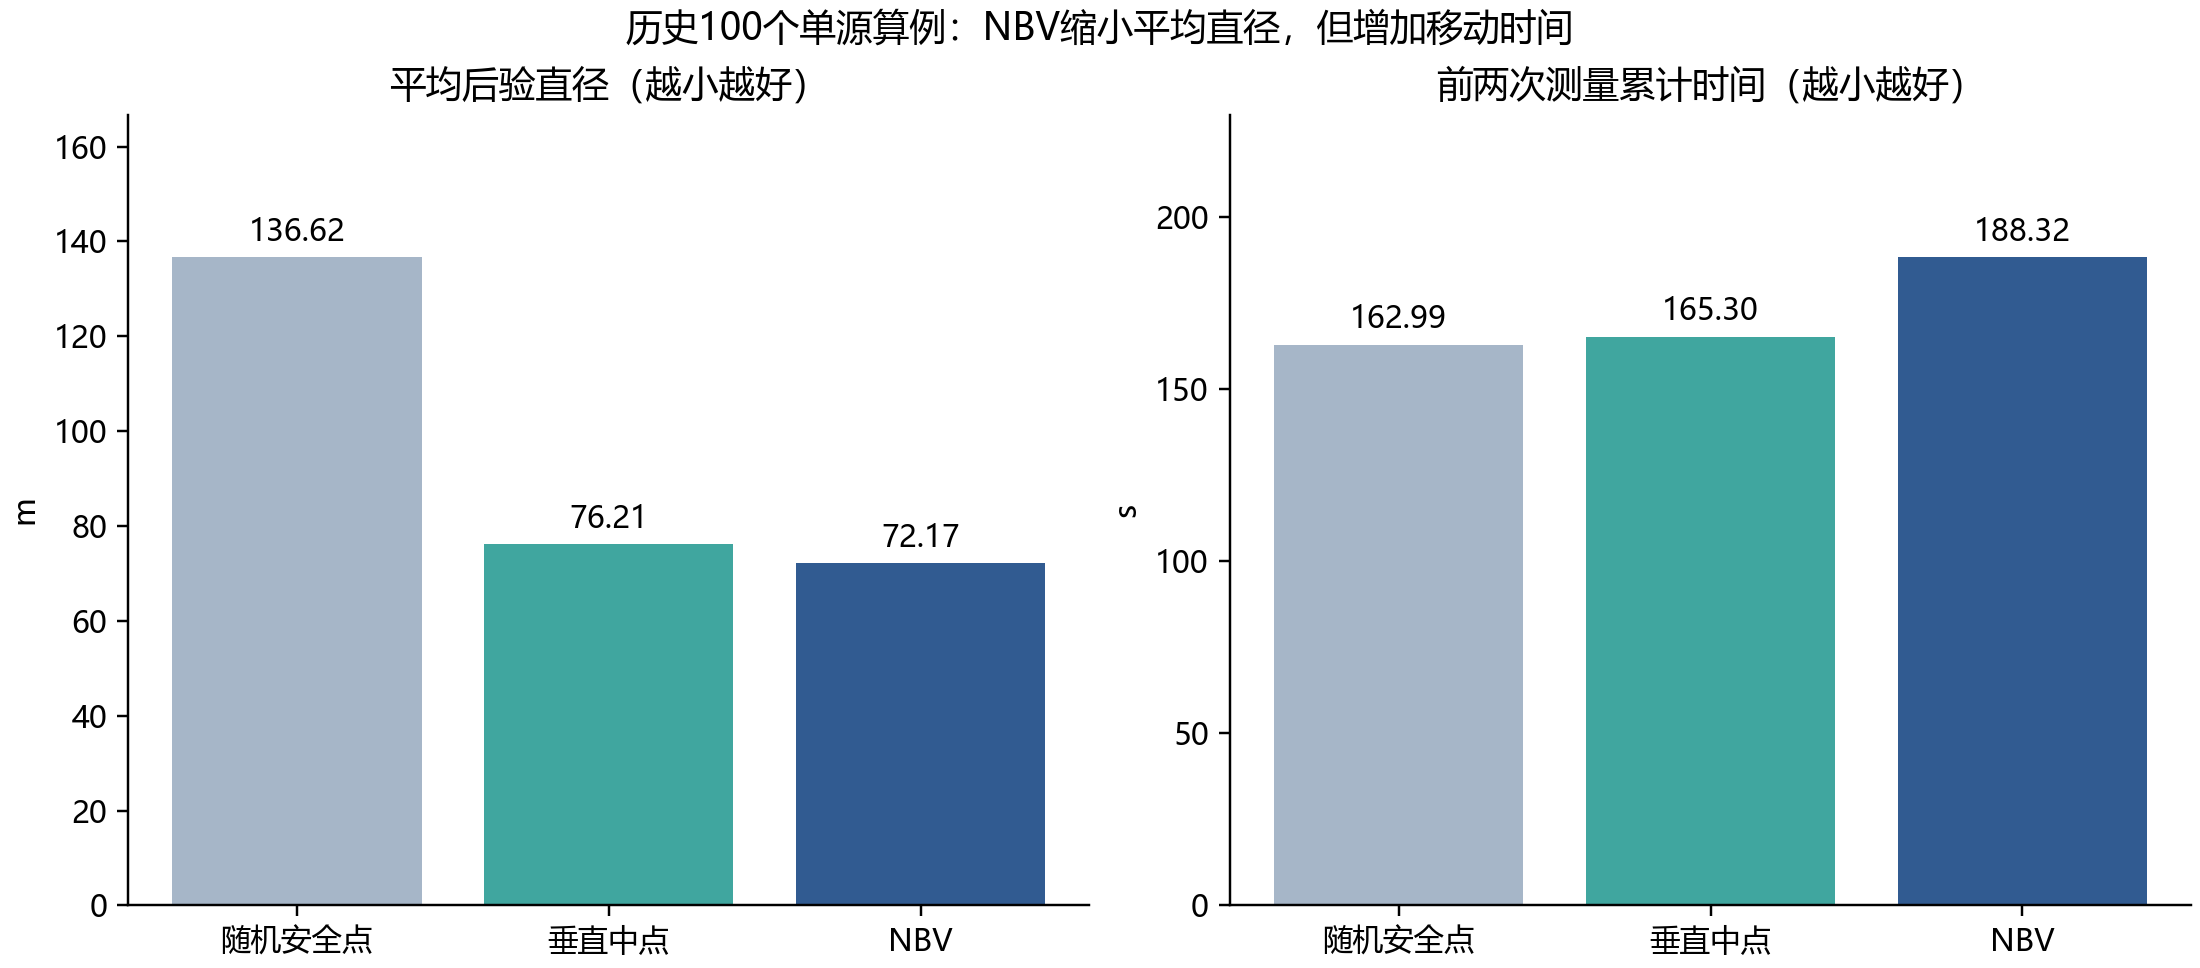
\includegraphics[width=0.98\textwidth]{figures/q2_historical_tradeoff.png}
 \caption{历史单源策略的定位尺度与时间代价。图由保存的300条记录重新汇总绘制，未新增模拟实验；两个纵轴分别使用米与秒，均从零开始。}
 \label{fig:q2-historical-tradeoff}
\end{figure}

由此需要进一步区分三类改进。首先，安全候选区域解决“是否能够收到信号”，这是相对无约束启发式的可行性加强，但会限制可选站位。其次，采样后验评分解决“哪些有限观测情景可能使定位区域收缩”，它在历史算例中降低了平均直径，却不保证每例都更好。最后，时间项显式暴露了几何收缩所付出的移动代价；固定 $213$ 个候选及其情景评分，再仅改变 $\lambda$，可得到表\ref{tab:q2-results}所示的可复核权重比较，而不会把候选生成器变化与时间权重变化混在一起。

在该固定候选算例中，将 $\lambda$ 从 $0.2$ 提高到 $1$，第二动作时间由 $204.29\,\mathrm s$ 降至 $184.29\,\mathrm s$，同时最大采样后验直径由 $112.92\,\mathrm m$ 增至 $130.45\,\mathrm m$；继续增大权重会进一步偏向短距离站位。该结果支持将时间作为可调决策偏好，而不支持宣称时间权重必然同时改善两个指标。上述验证将候选可行性、定位尺度与动作时间分开比较，使每项结论具有对应的证据和适用范围。

与问题一的清除证书对应，表\ref{tab:q1-stop-comparison}还显示，NBV 虽具有最小的平均后验直径，其第二次观测后的 MEC 就绪数却不是最多。这说明最小化平均定位尺度和尽快达到清除门槛并非等价目标；仅凭均值不能推断整局清除效率。当前方法保留“集合约束确保允许位置不被主动排除、证书控制清除、时间评分选择观测”的分工。其已有优势在于与有界误差和实际动作成本相容、每一决策量可复核；尚未得到连续最坏情景误差界或整局时间最优保证，面向后续清除时间的多步优化也不作为已经实现的收益。
